\documentclass[10pt,journal,compsoc]{IEEEtran}

\usepackage{grffile}
\usepackage[dvips]{graphicx}

\usepackage[cmex10]{amsmath}

\hyphenation{}

\begin{document}

\title{Eficiencia del sistema de propulsi\'on WARP de la nave espacial USS Enterprise}


\author{Lucila Stancato,~\IEEEmembership{I.T.B.A,}
		Dami\'an Modernell,~\IEEEmembership{I.T.B.A,}
		Juan Brasca,~\IEEEmembership{I.T.B.A,}
		Conrado Negro,~\IEEEmembership{I.T.B.A}%

}

\IEEEcompsoctitleabstractindextext{%
\begin{abstract}
%\boldmath
Analizamos la eficacia en la generaci\'on de n\'umeros pseudo-aleatorios del generador de L'Ecuyer aplicando los tests $\chi^2$ y $KS$
, en los que determinamos la conveniencia de usar dicho generador. Tambi\'en realizamos la estimaci\'on del tiempo
de vuelo de la nave espacial USS Enterprise mediante la simulaci\'on de Montecarlo.
\end{abstract}

\begin{IEEEkeywords}
Generador de L'Ecuyer, n\'umeros pseudoaleatorios, simulaci\'on de Montecarlo, propulsor WARP
\end{IEEEkeywords}
}%\IEEEcompsoctitleabstractindextext

\maketitle

\IEEEdisplaynotcompsoctitleabstractindextext

\IEEEpeerreviewmaketitle

\section{Introducci\'on}

\IEEEPARstart{L}{}os dispositivos de c\'omputo no pueden generar n\'umeros aleatorios dado que 
son dispositivos deterministas. La \'unica manera de obtenerlos ser\'ia a trav\'es de un dispositivo
que detecte procesos naturales como por ejemplo el intervalo de tiempo entre dos part\'iculas $\alpha$
en una muestra radiactiva.\\
En la secci\'on 2 utilizamos y sometemos a prueba el generador propuesto por L'Ecuyer para la
generaci\'on de n\'umeros pseudoaleatorios que a diferencia de los n\'umeros aleatorios, pueden 
ser generados por una computadora. En las distintas pruebas determinamos la bondad de ajuste del
generador. En la secci\'on 3 utilizamos el modelo de simulaci\'on de Montecarlo de sistemas
distribuidos para determinar el tiempo medio de vuelo y varianza del USS Enterprise.\\
Comprobamos la efectividad del generador de L'Ecuyer ya que genera n\'umeros que aparentan ser 
aleatorios.
sdafasdfasdfasdfasdfasdfasdfasdfasdfasdfasdfasdf

\section{Generador de L'Ecuyer}
El generador propuesto por L'Ecuyer en 1998 combina dos generadores lineales congruenciales (LCGs)
seg\'un los pasos del 1 al 5:
\begin{itemize}
 \item{PASO 1} Seleccionar una semilla $X_{1,0}$ en el rango $[1,2147483562]$ para el primer LCG y otra $X_{2,0}$ en el rango $[1,2147483398]$ para el segundo LCG.\\
 \item{PASO 2} Evaluar cada generador individual:
 \begin{align*}
  X_{1,n+1} &= 40014 X_{1,n} mod 2147483563\\
  X_{2,n+1} &= 40692 X_{2,n} mod 2147483399
 \end{align}
 
 \item{PASO 3} Computar:
 \begin{equation*}
  X_{n+1} = (X_{1,n+1} - X_{2,n+1}) mod 2147483562
 \end{equation}
 
 \item{PASO 4} Computar:
  \begin{equation*}
  \label{eq:f(t)}
  U_{n+1} = \left\{
  \begin{array}{rl}
	\frac{X_{n+1}}{2147483563} \hspace{0.5cm} 0 < X_{n+1}\\\\
	\frac{2147483562}{2147483563} \hspace{0.5cm} X_{n+1} = 0\\
  \end{array} \right.
  \end{equation}

 \item{PASO 5} Hcer $n = n + 1$ y volver al $PASO 2$
\end{itemize}

Los n\'umeros obtenidos por medio de este generador tienen una distribuci\'on uniforme.
Generamos 10000 n\'umeros que presentamos en el histograma de la figura 1.

\begin{figure}[t]
\label{fig:histogramalecuyer}
\begin{center}
\centering
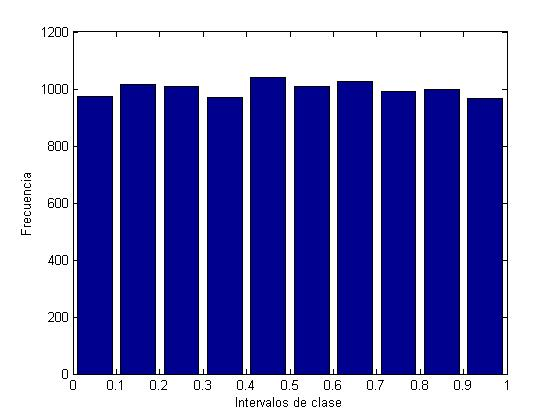
\includegraphics[width=3.2in]{clases.jpg}
\caption{10000 n\'umeros generados con el generador de L'Ecuyer divididos en 10 intervalos de clase que muestran una distribuci\'on uniforme}
\end{center}
\end{figure}

Analizamos gr\'aficamente en el plano las duplas $(U_i, U_{i+1})$ en la figura 2 y en el espacio las ternas $(U_i, U_{i+1}, U_{i+2})$ en la figura 3.

\begin{figure}[t]
\label{fig:2d}
\begin{center}
\centering
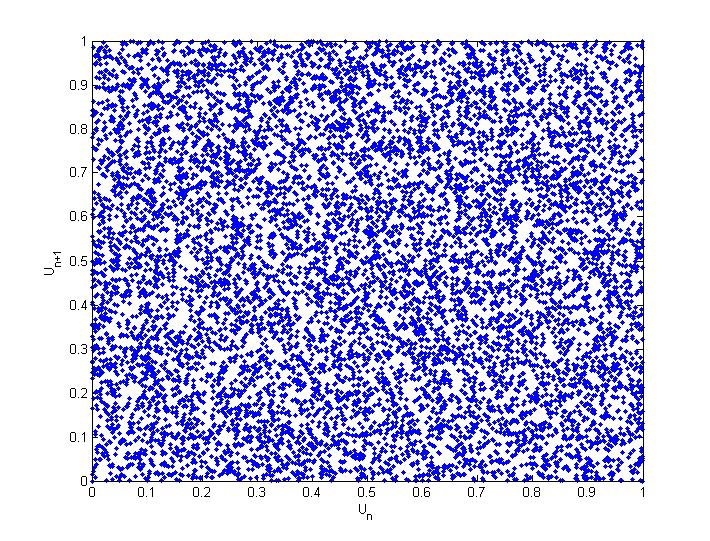
\includegraphics[width=3.2in]{2d.jpg}
\caption{Observamos la distribuci\'on uniforme de los 10000 n\'umeros obtenidos con el generador de L'Ecuyer}
\end{center}
\end{figure}

\begin{figure}[t]
\label{fig:3d}
\begin{center}
\centering
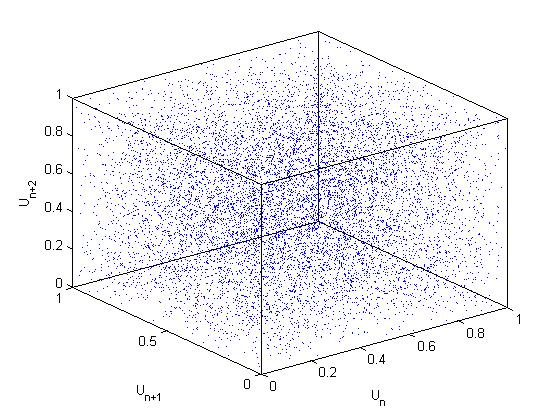
\includegraphics[width=3.2in]{3d.jpg}
\caption{Observamos la distribuci\'on uniforme de los 10000 n\'umeros obtenidos con el generador de L'Ecuyer}
\end{center}
\end{figure}

\subsection{Prueba $\chi^2$}

\subsection{Prueba de Kolmogorov-Smirnov}


\section{parte b}

\section{algoritmo funcion triangular}

\section{Simulacion de montecarlo del enterprise}



%\begin{figure}[t]
%\label{fig:refuerzos2}
%\begin{center}
%\centering
%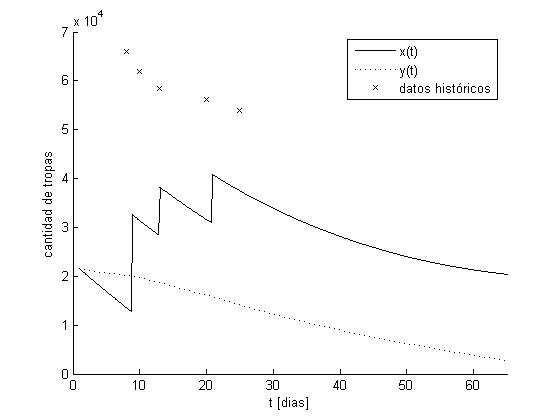
\includegraphics[width=3.2in]{grafico3_bis}
% where an .eps filename suffix will be assumed under latex, 
% and a .pdf suffix will be assumed for pdflatex; or what has been declared
% via \DeclareGraphicsExtensions.
%\caption{Segunda politica de refuerzos}
%\end{center}
%\end{figure}
%
%\begin{figure*}[!t]
%\centerline{\subfloat[Case I]\includegraphics[width=2.5in]{subfigcase1}%
%\label{fig_first_case}}
%\hfil
%\subfloat[Case II]{\includegraphics[width=2.5in]{subfigcase2}%
%\label{fig_second_case}}}
%\caption{Simulation results}
%\label{fig_sim}
%\end{figure*}

\section{Conclusi\'on}

\begin{thebibliography}{1}

\bibitem{IEEEhowto:kopka}
D\'iaz, A. R. \emph{El concepto de control}. Departamento de Ingenier\'ia Informatica. 
Instituto Tecnol\'ogico de Buenos Aires.
\end{thebibliography}

\end{document}


